% Условная компиляция для самостоятельной работы
\ifdefined\mainfile
    % Если это часть основного файла, не добавляем начало и конец документа
\else
    \documentclass[12pt, a4paper]{report}
    \usepackage{/Users/vladbelousov/Desktop/Semestr_4-FP-NSU/Настройка/library}
    \usepackage[utf8]{inputenc} % Подключение поддержки UTF-8
    \begin{document}
\fi

%%-------------------------------%%

\section{Классическая теория дисперсии света в среде}

Модель взаимодействия среды с электромагнитной волной: разряженный холодный газ атомов: 

1) Частицы газа не взаимодействуют 

2) Поле, действующее на атомы, совпадают со средним полем в среде

3) Действием магнитного поля пренебрегаем 

Электроны в атоме можно приближенно разделить на: слабосвязанные (оптические), эффективно взаимодействующие с электромагнитными волнами оптического диапазона  и сильно связанные, которые слабо взаимодействуют с этими частицами 
\begin{center}
    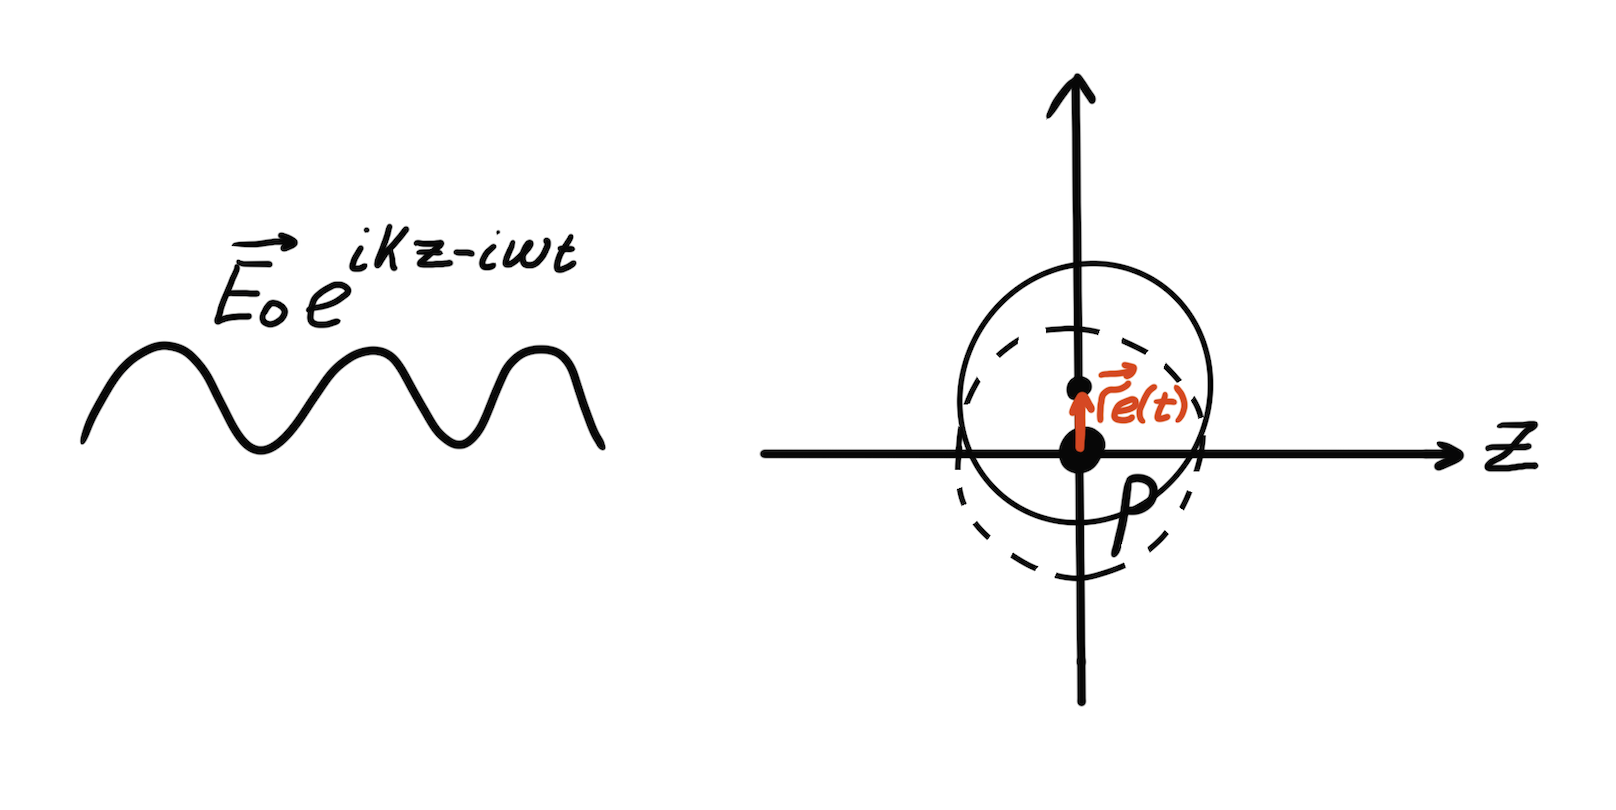
\includegraphics[width=0.6\textwidth]{/Users/vladbelousov/Desktop/Semestr_4-FP-NSU/ЭиО/Лекции_по_дням/image/34.png}
\end{center}
\[ \vec{F}_{e \to p } = \frac{4}{3 }  \pi \underbrace{\rho_e}_{ \rho = \frac{e}{\frac{4 }{3 }  \pi a ^3 } } (- \vec{r }_e (t ) )|e|   \] 

\[\Rightarrow \vec{F } _e = - \frac{e |e|}{a ^3 } \vec{r}_e (t ) = - \frac{e^2 }{a^3 } \vec{r } _e (t )      \] 

\[ \vec{F } _{p \to  e } = - \vec{ F } _{e \to  p } = - \frac{e ^2 } { a ^3 }\vec{r } _e (t )    \] 

\[ m\ddot{\vec{r}  }_e = e \vec{E }  _0 e ^{- i \omega t } - \frac{e^ 2 }{a ^3 }   \vec{r } _e(t ) +\vec{F } _{\text{трен} }    \] 

\[ \ddot{\vec{r } }_e + \underbrace{\frac{e ^2 }{m a^ 3}}_{= \omega_0 ^2 } \vec{r } _e +\underbrace{2 \gamma \dot{\vec{r } }_e}_{\frac{\text{сила трения} }{m} } = \frac{e \vec{E } _0 }{m }e^{- i \omega t }  -\text{вынужденные колебания}    \] 

\[ \vec{r        }_e  = \vec{r_0 } e^{- i \omega t }    \] 

\[ \vec{r } _{0 } ( -\omega ^2 ) + \omega_0^2 \vec{r } _0 - 2 i \gamma \omega \vec{r_0} \Rightarrow \vec{r_0 } = \frac{e \vec{E_0 } }{m } \frac{1}{\omega_0 ^2 - \omega ^2 - 2 i \gamma \omega}      \] 

\[ \vec{r_e } (t )  =\frac{e \vec{E_0 } }{m }\frac{1}{\omega_0 ^2 - \omega ^2 - 2 i \gamma \omega} e^{- i \omega t }    \] 

Далее: \( \displaystyle \vec{D }  = \vec{E }  +4 \pi \vec{P }  , \quad  \vec{P }  = n_e \vec{d }_e = n_e e \vec{r } _e (t ) \) 

\[ \vec{D }  = \vec{E }  _0 e^{ -i \omega t } + 4 \pi n_e \frac{e \vec{E } _0 }{m } \frac{1}{\omega_0 ^2 - \omega ^2 - 2 i \gamma \omega} e^{- i \omega t }  = \underbrace{\left(  1+ \overbrace{\frac{4 \pi n_e e ^2 } { m }}^{\omega_p ^2 } \frac{1}{\omega_0 ^2 - \omega ^2 -  2 i \gamma \omega  }\right) }_{\varepsilon ( \omega)}\underbrace{\vec{E }  _0 e^{- i \omega t }}_{\vec{E }(t ) }     \] 

1 случай: Дисперсия вдали от линии поглощения 

\[ |\omega_0 ^2 - \omega ^2 | \gg 2 \gamma \omega  \] 

Уравнение дисперсионное соотношение: \( \displaystyle \frac{\omega \sqrt{\varepsilon ( \omega )\mu ( \omega )}}{c } = k , \mu (\omega ) = 1   \) 

\[ \varepsilon (\omega ) \simeq 1+ \frac{\omega_p ^2 } { \omega_0 ^2 - \omega ^2 } \Rightarrow n ( \omega ) \simeq \sqrt{\varepsilon (\omega )} \simeq 1+ \frac{\omega_p ^2 } {2(\omega_0 ^2 - \omega ^2) }       \] 

\begin{center}
    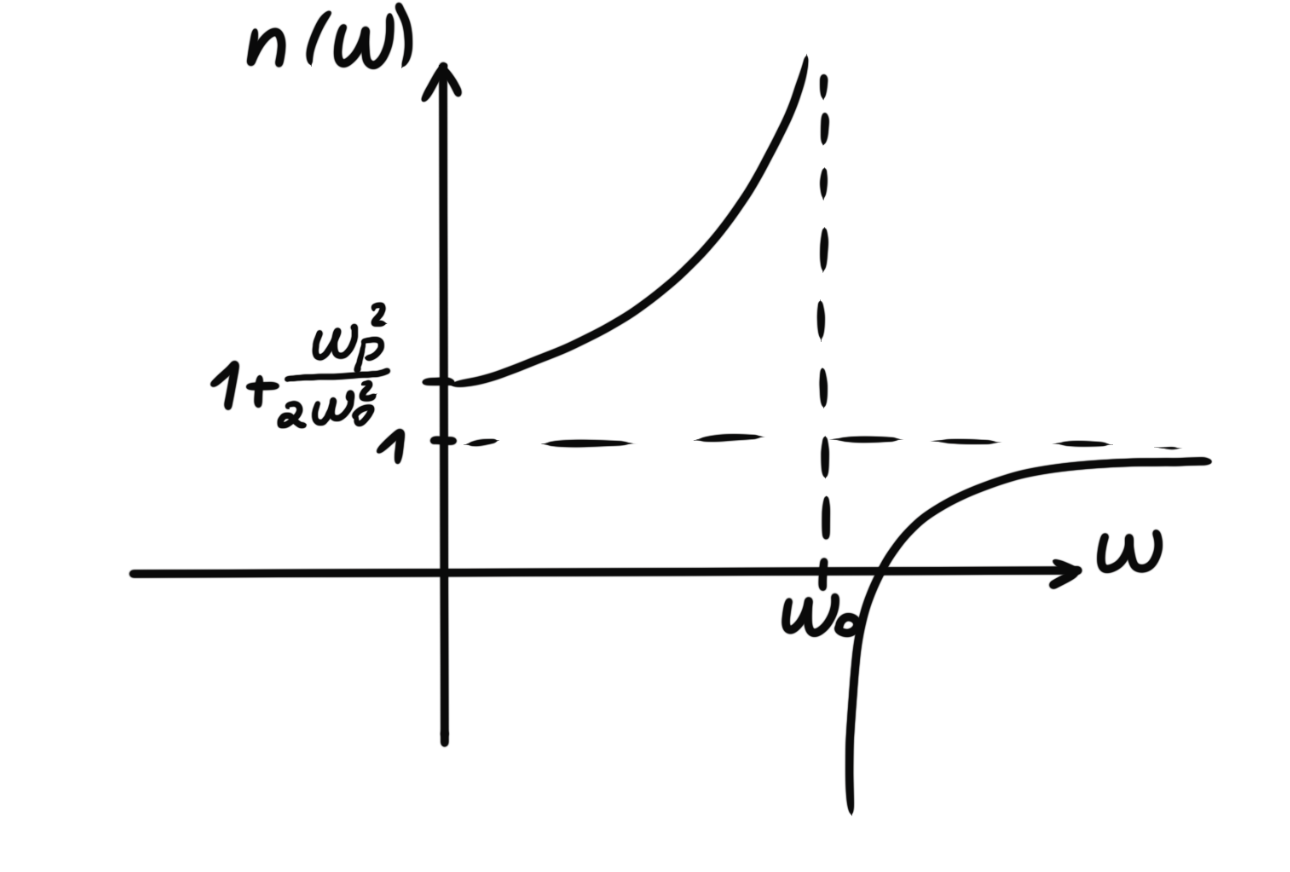
\includegraphics[width=0.6\textwidth]{/Users/vladbelousov/Desktop/Semestr_4-FP-NSU/ЭиО/Лекции_по_дням/image/35.png}
\end{center}

\[ \frac{dn ( \omega)}{d \omega} > 0 - \text{ нормальная дисперсия }: v_{g } < v_{\Phi }     \] 

2 случай: Дисперсия вблизи линии поглощения \( \omega \simeq \omega_0  \) 

\[ \omega = \omega_0 \Delta \omega , \quad  \Delta \omega \ll \Rightarrow \omega_0 ^2 - ( \omega+ \Delta \omega ) ^2 - 2 i \gamma ( \omega_0 + \Delta \omega ) = -2 \omega_0 \Delta \omega - \Delta \omega ^2 - 2 i \gamma \omega_0 - 2 i \gamma \Delta\omega   \] 

\[ \varepsilon ( \omega ) \simeq 1 - \frac{ \omega_p ^2 }{2 \omega_0 (\Delta \omega + i \gamma)}; \quad  n( \omega ) = \sqrt{\varepsilon( \omega)} \simeq 1 \frac{ \omega_p ^2 }{4 \omega_0 (\Delta \omega + i \gamma)} \frac{ \Delta \omega - i \gamma }{\Delta \omega - i \gamma} =     \] 

\[ =1  -\frac{\omega_p ^2 \Delta \omega}{4 \omega_0 (\Delta \omega ^2 + \gamma ^2)} + i \frac{ \omega_p ^2 \gamma }{4 \omega_0(\Delta \omega ^2 + \gamma ^2) }= 1- \frac{ \omega_p ^2 }{4 \omega_0 \gamma }\frac{ ( \frac{\Delta \omega}{\gamma} )}{1+ \left( \frac{\Delta \omega}{\gamma}  \right) ^2 } + i \frac{\omega_p ^2 }{4 \omega_0\gamma } \frac{ 1}{1+ \left( \frac{\Delta \omega}{\gamma}  \right) ^2}    \] 

\begin{center}
    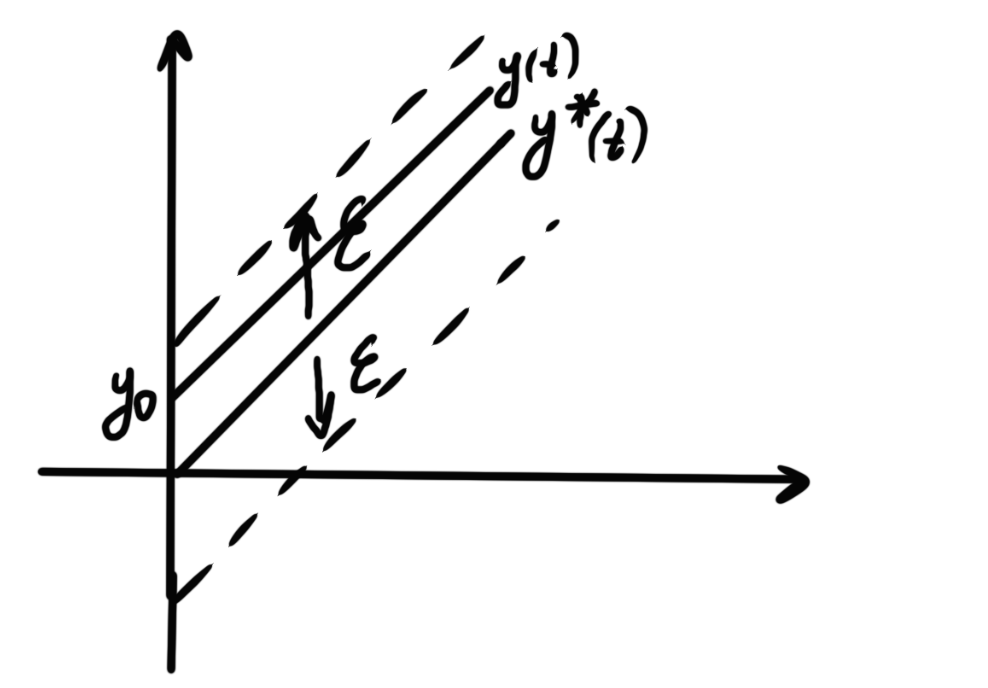
\includegraphics[width=0.45\textwidth]{/Users/vladbelousov/Desktop/Semestr_4-FP-NSU/ЭиО/Лекции_по_дням/image/36.png}
    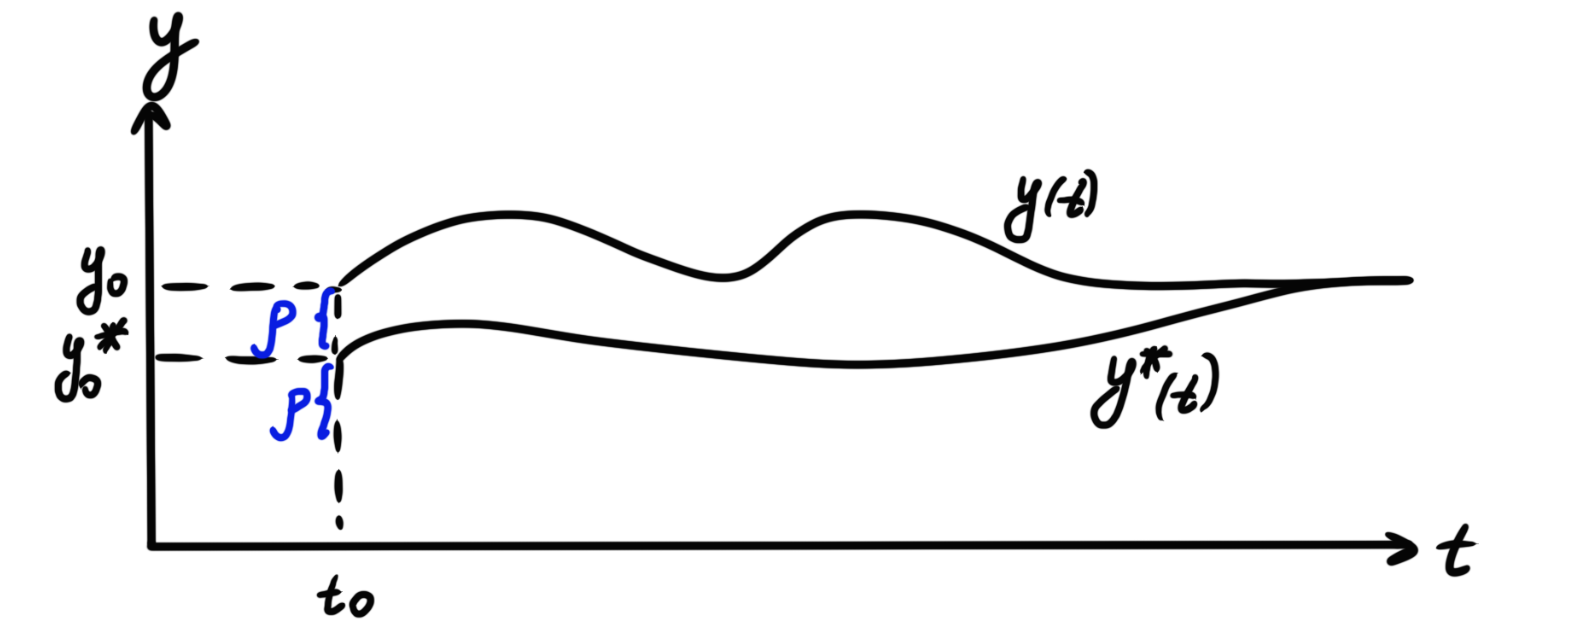
\includegraphics[width=0.45\textwidth]{/Users/vladbelousov/Desktop/Semestr_4-FP-NSU/ЭиО/Лекции_по_дням/image/37.png}
\end{center}

\[ k = \frac{\omega}{c }  \sqrt{ \varepsilon ( \omega )} = \frac{ \omega n ( \omega )}{c }  = \frac{\omega}{ c } \mathrm{Re } (n (\omega))+ \frac{i \omega}{c } \mathrm{Im }  (n (\omega))    \] 

\begin{center}
    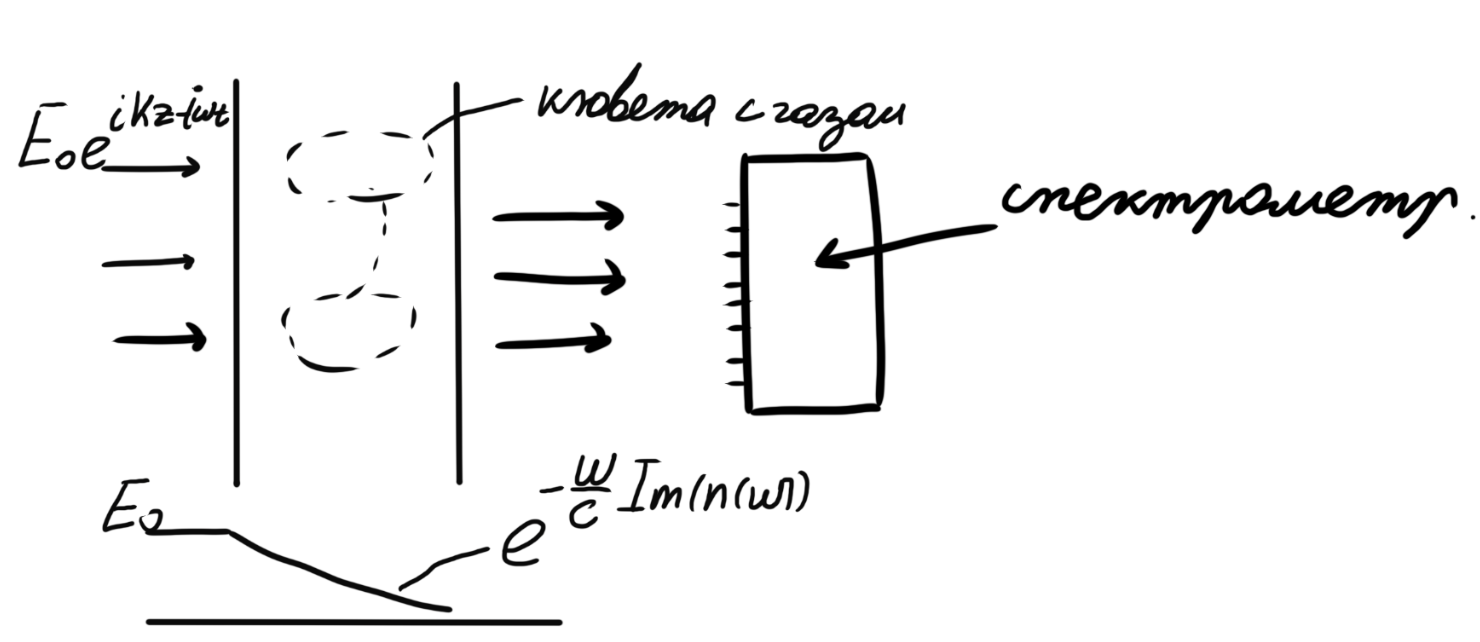
\includegraphics[width=0.6\textwidth]{/Users/vladbelousov/Desktop/Semestr_4-FP-NSU/ЭиО/Лекции_по_дням/image/38.png}
\end{center}

\[ \vec{E } (z, t ) = \vec{E } _ 0 e ^{ i \frac{\omega}{c } \mathrm{Re } (n ( \omega )) - i \omega t  } e^{- \frac{\omega}{ c } \mathrm{Im } (n ( \omega )) z  } \] 

Показания спектрометра: 

\begin{center}
    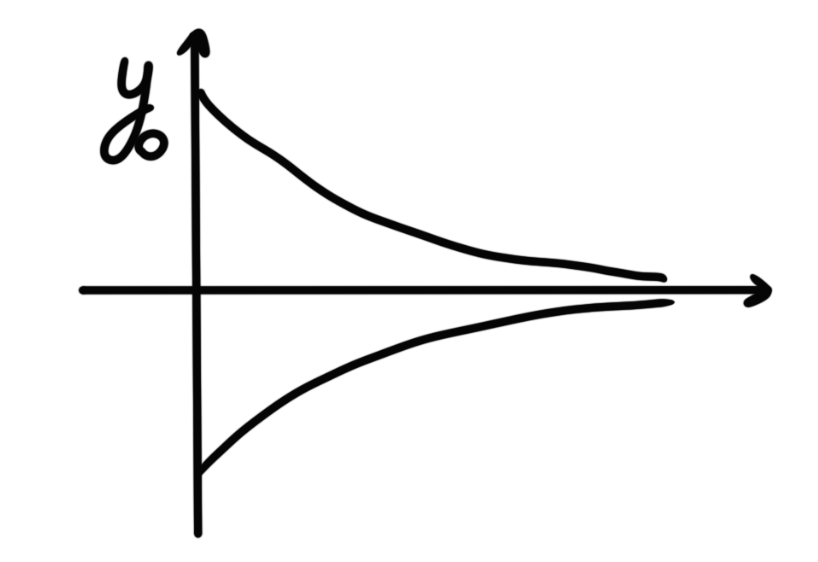
\includegraphics[width=0.6\textwidth]{/Users/vladbelousov/Desktop/Semestr_4-FP-NSU/ЭиО/Лекции_по_дням/image/39.png}
\end{center}

В квантовой теории \(\displaystyle  \varepsilon ( \omega ) = 1 + \frac{3 \pi Na e ^2 }{m } \sum_{n=1}^{\infty  } \frac{f_n }{\omega_{on } ^2 - \omega ^2 -2 i \gamma_n \omega }    \) 

\begin{center}
    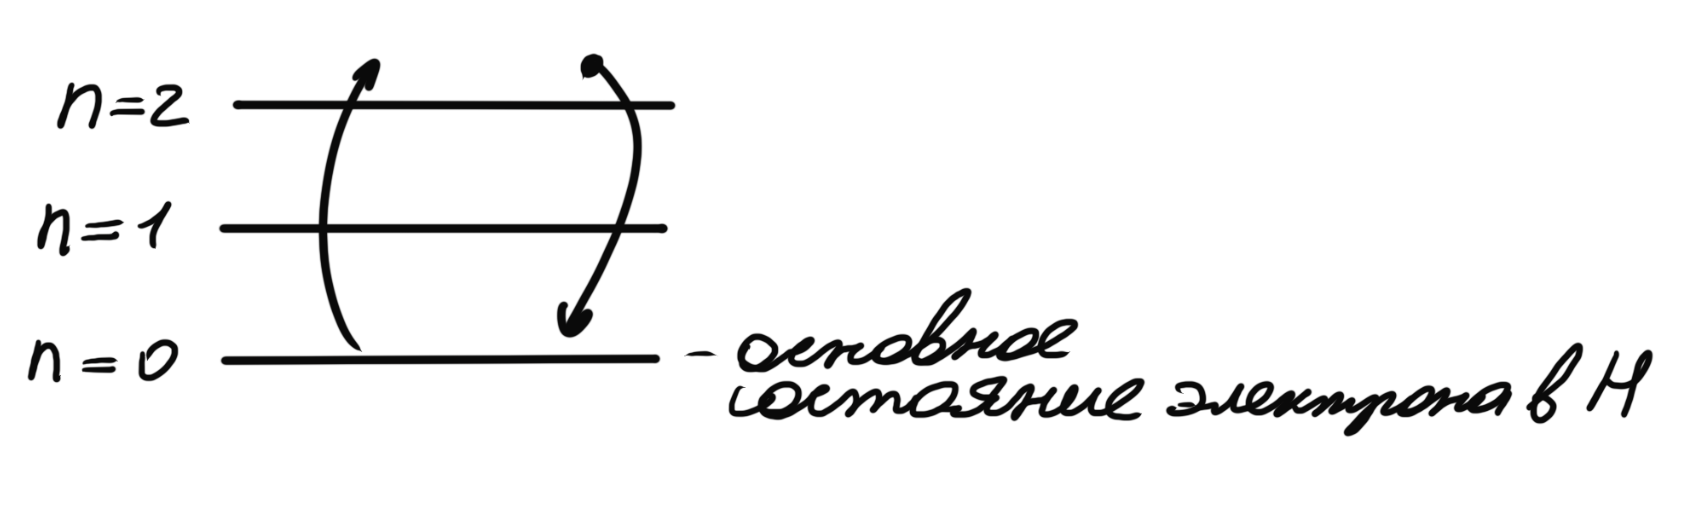
\includegraphics[width=0.6\textwidth]{/Users/vladbelousov/Desktop/Semestr_4-FP-NSU/ЭиО/Лекции_по_дням/image/40.png}
\end{center}

\[ h \omega _{on     } = \varepsilon_n -\varepsilon_0 - \text{энергия перехода с n-го уровня на основной} ,\quad  h = 1,054 \cdot 10 ^{-27} \text{эрг с }    \]  

\[ f_n - \text{сила осциллятора - вероятность перехода с n-го уровня на основной  } \Rightarrow \sum_{n =1} ^{\infty  } f_n = 1   \] 

\section{ Стоячие волны}

\begin{center}
    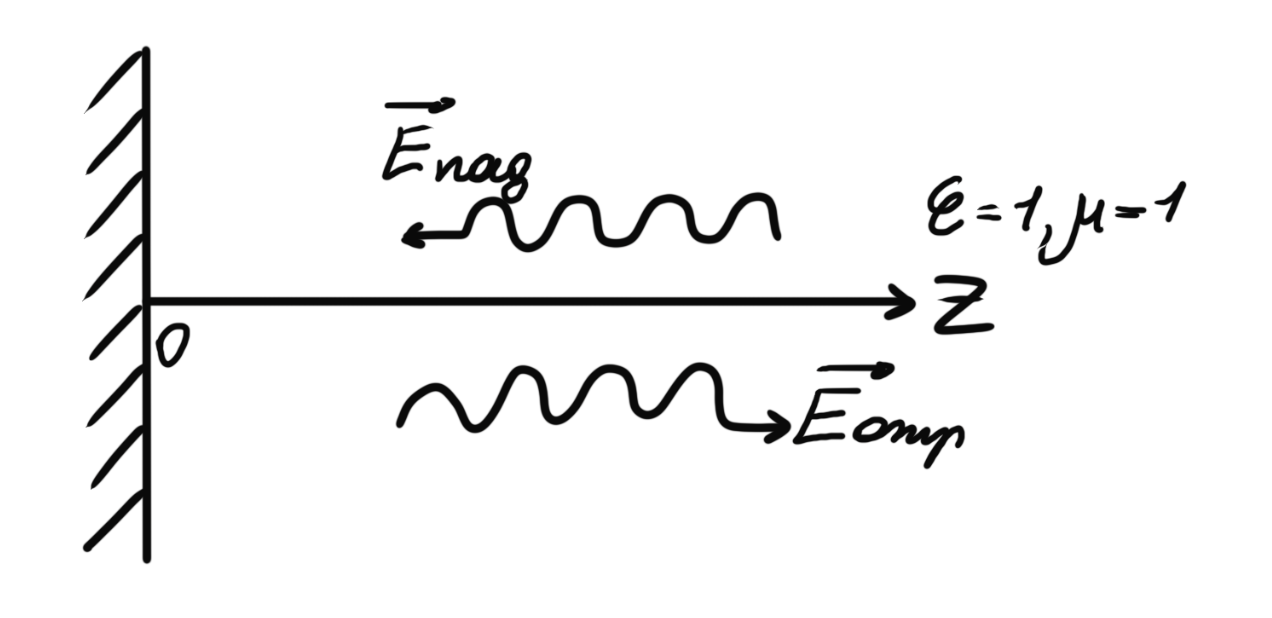
\includegraphics[width=0.6\textwidth]{/Users/vladbelousov/Desktop/Semestr_4-FP-NSU/ЭиО/Лекции_по_дням/image/41.png}
\end{center}

\[ \vec{E } _{\text{пад } } =   \vec{E }  _ 0 e^{i (\vec{k},\vec{r }     )- i \omega t }  = \vec{E } _0 e^{- i k z - i \omega t } \quad ( \vec{E } _0 \perp \vec{n }  = - \vec{e } _z ), \quad \vec{k } = \vec{n } k = - \vec{e }_z k\] 

\[ \vec{E } _{\text{отр }  } = \vec{E } _1 e^{i kz - i \omega t }, \quad  \vec{E } _1 \perp \vec{e }_z     \] 

Граничные условия на поверхности проводника

\[ \vec{E } , \vec{\tau }_{\text{Г } } = 0 , \quad E_{\tau } =( \vec{E } _ 0 ,\vec{\tau } )+ ( \vec{E } _ 1 , \vec{\tau } ) = 0 = ((\vec{E } _0 + \vec{E } _1), \vec{\tau } )= 0      \] 

\[ \Rightarrow \vec{E_0} + \vec{E_1 } = 0 \Rightarrow \vec{E_0 } = -\vec{E_1}      \] 

\[ \vec{E}_{\Sigma } = \vec{E_0 }e^{ - i kz - i\omega t}  - \vec{E_0 }e^{i kz - i \omega t } = \vec{E_0 }e^{- i \omega t } \frac{ e^{- ikz } - e^{i kz } }{2i } 2 i= -2i \vec{E_0 }\sin (kz) e^{- i \omega t }          \] 

\[ \vec{B }  = \vec{H }  = \sqrt{\frac{ \varepsilon }{\mu } } [ \vec{n } \times  \vec{E } ]  \]

\[ \vec{B }_{\text{пад } } = [ - \vec{e } _z \times  \vec{E_0}  ]   e^{- ikz - i \omega t } , \quad  \vec{B }_{\text{отр } } = [  \vec{e } _z \times  (-\vec{E_1 }) ] e^{ikz - i \omega t } \] 

1 пример: падающая волна линейно поляризована 

\[ \vec{E_0 } = \vec{e_x  }|c_1         | e^{i \varphi } , \text{ }  c_1 \in \mathbb{C} ; \text{ } \mathrm{Re }  (\vec{E }_{\Sigma }( z, t ))  = - 2 |c_1 | \vec{e } _x \sin(kz ) \sin (\omega t  - \varphi )        \] 

\[ \mathrm{Re } (\vec{B } _{\Sigma } (z, t ) ) = - 2 \vec{e }  _{y }  \cos ( kz ) \cos  ( \omega t - \varphi ) |c_1 | \] 

\begin{center}
    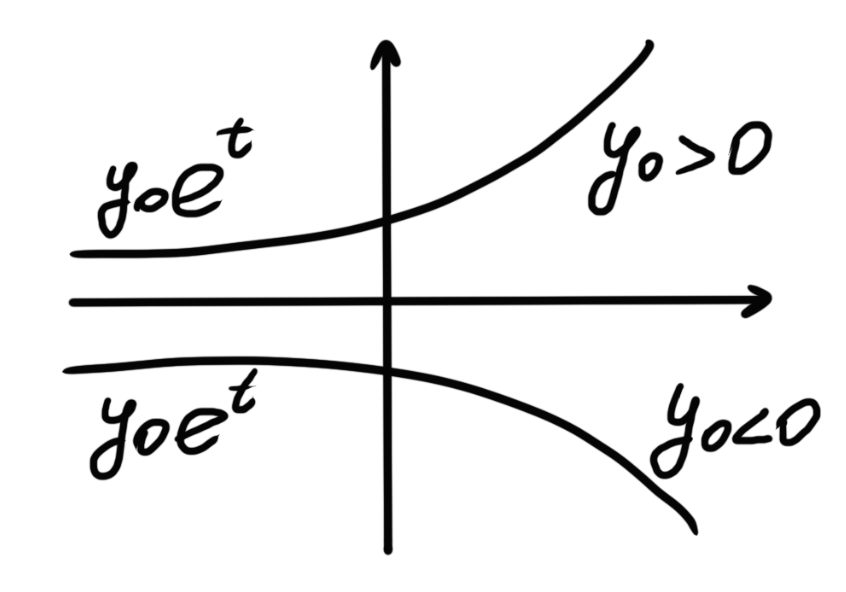
\includegraphics[width=0.6\textwidth]{/Users/vladbelousov/Desktop/Semestr_4-FP-NSU/ЭиО/Лекции_по_дням/image/42.png}
\end{center}
Узлы: \( k z_{m }= m \pi , z_{m }  = \frac{m \lambda }{2 } \) 


Пучность: \( k z_{m } ' = m \pi + \frac{\pi}{2 } , \quad  z_m ' = \frac{ m \pi + \frac{\pi}{2} }{k } = \frac{m \lambda }{2} + \frac{\lambda}{ 4 }    \) 

2 пример: круговая поляризация \( \vec{E } _0 = ( \vec{e } _ x + i \vec{e } _ y ) |c_1 |e^{ i \varphi} - \text{левая круговая}  \) 

\[ \mathrm{Re } (\vec{E } _{\Sigma }(z, t ) ) = \mathrm{Re }  \left[ -2 i ( \vec{e } _ x + i \vec{e }  _ y )|c_1|e^{- i ( \omega t - \varphi )} \sin (kz)  \right]= -2 |c_1 | \sin (kz) [\vec{e } _ x \sin (\omega t - \varphi) - \vec{e } _y \cos (\omega t - \varphi )]  \] 

\[ \mathrm{Re } (\vec{B }_{\Sigma }( z, t )  ) =2 |c_1 | \cos (kz) [\vec{e } _ x \sin (\omega t - \varphi) - \vec{e } _y \cos (\omega t - \varphi )]   \] 

%%-------------------------------%%

% Закрытие документа, если файл компилируется отдельно
\ifdefined\mainfile
    % Если это основной файл, не нужно заканчивать документ
\else
    \end{document}
\fi